\documentclass[10pt,english]{article}

%\usepackage[T1]{fontenc}
%\usepackage[utf8]{inputenc}
\usepackage[a4paper,left=0.4in, right=0.4in,top=0.5in,bottom=0.6in]{geometry}
\usepackage{amsmath}
\usepackage{amssymb}
\usepackage{subcaption}
\usepackage{epstopdf}
\usepackage{graphicx}
\usepackage{mathrsfs}
\usepackage{epstopdf}
\usepackage{mathtools}
\usepackage{textcomp}
\usepackage{graphicx}
\usepackage{xcolor}
\usepackage{epstopdf}
%\usepackage{multicol}
%\usepackage{tikz}
\usepackage{hyperref}

% code listing settings
\usepackage{listings}
\lstset{
    language=Python,
    basicstyle=\ttfamily\small,
    aboveskip={1.0\baselineskip},
    belowskip={1.0\baselineskip},
    columns=fixed,
    extendedchars=true,
    breaklines=true,
    tabsize=4,
    prebreak=\raisebox{0ex}[0ex][0ex]{\ensuremath{\hookleftarrow}},
    frame=lines,
    showtabs=false,
    showspaces=false,
    showstringspaces=false,
    keywordstyle=\color[rgb]{0.627,0.126,0.941},
    commentstyle=\color[rgb]{0.133,0.545,0.133},
    stringstyle=\color[rgb]{01,0,0},
    numbers=left,
    numberstyle=\small,
    stepnumber=1,
    numbersep=10pt,
    captionpos=t,
    escapeinside={\%*}{*)}
}
\author{Steven Porretta \\ Student \# 100756494}
\title{Assignment \#4}
\date{}
\begin{document}
    \maketitle
    Code can be found at \url{https://github.com/0xSteve/learning_automata_simulator}
    \section{Question 1}
        In this section we will examine some code snippets from the first question.
    \begin{lstlisting}[label={list:first},caption=Testbench code for the Tsetlin.] 
    c2 = 0.7
    c1 = 0.05
    for i in range(0, 7):
        print("c1 = " + str(c1) + ", c2 = " + str(c2) + ", N = 13.")
        a = la.Tsetlin(13, 2, [c1, c2])
        a.simulate(50, 30001)
        b = ala.Tsetlin.stationary_probability_analytic([c1, c2], 13)
        c = ala.Tsetlin.number_of_states_estimate([c1, c2])
        print("Tsetlin P1(infinity) = " + str(b) + "(Analytic)")
        print("Tsetlin P1(infinity) = " + str(a.action_average[0]) + "(Simulated)")
        print("Tsetlin # of states required = " + str(c) + "(Estimate)")
        c1 += 0.1
        c1 = round(c1, 2)
\end{lstlisting}
This excerpt of code generates the entire quantity of required code for this question.  As can be seen in the following code-snippet.

\begin{lstlisting}[label={list:first},caption=Testbench output.] 
c1 = 0.05, c2 = 0.7, N = 13.
Tsetlin P1(infinity) = 0.9999999890725503(Analytic)
Tsetlin P1(infinity) = 1.0(Simulated)
Tsetlin # of states required = 3(Estimate)
c1 = 0.15, c2 = 0.7, N = 13.
Tsetlin P1(infinity) = 0.9999778874501014(Analytic)
Tsetlin P1(infinity) = 1.0(Simulated)
Tsetlin # of states required = 4(Estimate)
c1 = 0.25, c2 = 0.7, N = 13.
Tsetlin P1(infinity) = 0.9990142374252533(Analytic)
Tsetlin P1(infinity) = 0.999998000067(Simulated)
Tsetlin # of states required = 6(Estimate)
c1 = 0.35, c2 = 0.7, N = 13.
Tsetlin P1(infinity) = 0.9865794150962881(Analytic)
Tsetlin P1(infinity) = 0.999797340089(Simulated)
Tsetlin # of states required = 9(Estimate)
c1 = 0.45, c2 = 0.7, N = 13.
Tsetlin P1(infinity) = 0.9151468144874294(Analytic)
Tsetlin P1(infinity) = 0.980783973868(Simulated)
Tsetlin # of states required = 18(Estimate)
c1 = 0.55, c2 = 0.7, N = 13.
Tsetlin P1(infinity) = 0.7453193640776348(Analytic)
Tsetlin P1(infinity) = 0.786514449518(Simulated)
Tsetlin # of states required = 0(Estimate)
c1 = 0.65, c2 = 0.7, N = 13.
Tsetlin P1(infinity) = 0.5680008401435711(Analytic)
Tsetlin P1(infinity) = 0.570874970834(Simulated)
Tsetlin # of states required = 0(Estimate)
\end{lstlisting}
Now that it is seen working as one would expect, considering rounding errors from python 3.6, it is time to take a look at the useful snippets of code governing the functionality of the Tsetlin, and Krylov automata.

\begin{lstlisting}[label={list:first},caption=Tsetlin core code.] 
     def next_state_on_reward(self):
        '''Find the next state of the learner, given that the teacher
           rewarded.'''
        if (self.current_state mod (self.N / self.R) != 1):
            self.current_state -= 1

    def next_state_on_penalty(self):
        '''Find the next state of the learner, given that the teacher
           penalized.'''
        if(self.current_state mod (self.N / self.R) != 0):
            self.current_state += 1
        elif(self.current_state mod (self.N / self.R) == 0):
            # Don't really add states, just cycle through N, 2N, 4N, etc.
            if(self.current_state != self.N):
                a = (self.N / self.R) mod self.N
                self.current_state = a + self.current_state
            else:
                self.current_state = self.N / self.R

    # Determine the next state as the teacher.
    def environment_response(self):
        '''Determine the next state of the learner from the perspective
        of the teacher.'''
        response = uniform(0, 1)
        penalty_index = 1
        if(self.current_state <= self.n):
            self.actions[0] += 1
            penalty_index = 0
        else:
            self.actions[1] += 1

        if(response > self.c[penalty_index]):
            # Reward.
            self.next_state_on_reward()
        else:
            # Penalty.
            self.next_state_on_penalty()
\end{lstlisting}
The above is the core code of the Tsetlin machine, governing state translations and action choices.  Essentially, whenever it is in the range 1 to N, it chooses action $\alpha_1$ and $\alpha_2$ otherwise.  This code is essentially the same for the Krylov machine, which we will see in the next section.

\section{Question 2}
\begin{lstlisting}[label={list:first},caption=testbench for the Krylov 2-action.] 
    for i in range(0, 7):
    print("c1 = " + str(c1) + ", c2 = " + str(c2) + ", N = 13.")
    a = la.Tsetlin(13, 2, [c1/2, c2/2])
    a.simulate(50, 30001)
    b = ala.Tsetlin.stationary_probability_analytic([c1, c2], 13)
    c = ala.Tsetlin.number_of_states_estimate([c1, c2])
    d = la.Krylov(13, 2, [c1, c2])
    d.simulate(10, 50000)
    e = ala.Tsetlin.stationary_probability_analytic([c1, c2], 13)
    f = ala.Tsetlin.number_of_states_estimate([c1, c2])
    print("Tsetlin P1(infinity) = " + str(b) + "(Analytic)")
    print("Tsetlin P1(infinity) = " + str(a.action_average[0]) + "(Simulated)")
    print("Tsetlin # of states required = " + str(c) + "(Estimate)")
    print("Krylov P1(infinity) = " + str(e) + "(Analytic)")
    print("Krylov P1(infinity) = " + str(d.action_average[0]) + "(Simulated)")
    print("Krylov # of states required = " + str(f) + "(Estimate)")
    c1 += 0.1
    c1 = round(c1, 2)
\end{lstlisting}
As can be seen from the code, this test bench looks very similar to the test bench of question 1, however, note the $c$ vector for the Tsetlin automaton is now $c_1 / 2 $, $c_2/2$.  As is expected, both automata behave in the same manner. as can be seen from the output code snippet.
\begin{lstlisting}[label={list:first},caption=testbench output for the Krylov 2-action.] 
    c1 = 0.05, c2 = 0.7, N = 13.
    Tsetlin P1(infinity) = 0.9999999890725503(Analytic)
    Tsetlin P1(infinity) = 1.0(Simulated)
    Tsetlin # of states required = 3(Estimate)
    Krylov P1(infinity) = 0.9999999890725503(Analytic)
    Krylov P1(infinity) = 1.0(Simulated)
    Krylov # of states required = 3(Estimate)
    c1 = 0.15, c2 = 0.7, N = 13.
    Tsetlin P1(infinity) = 0.9999778874501014(Analytic)
    Tsetlin P1(infinity) = 0.999999333356(Simulated)
    Tsetlin # of states required = 4(Estimate)
    Krylov P1(infinity) = 0.9999778874501014(Analytic)
    Krylov P1(infinity) = 1.0(Simulated)
    Krylov # of states required = 4(Estimate)
    c1 = 0.25, c2 = 0.7, N = 13.
    Tsetlin P1(infinity) = 0.9990142374252533(Analytic)
    Tsetlin P1(infinity) = 1.0(Simulated)
    Tsetlin # of states required = 6(Estimate)
    Krylov P1(infinity) = 0.9990142374252533(Analytic)
    Krylov P1(infinity) = 1.0(Simulated)
    Krylov # of states required = 6(Estimate)
    c1 = 0.35, c2 = 0.7, N = 13.
    Tsetlin P1(infinity) = 0.9865794150962881(Analytic)
    Tsetlin P1(infinity) = 1.0(Simulated)
    Tsetlin # of states required = 9(Estimate)
    Krylov P1(infinity) = 0.9865794150962881(Analytic)
    Krylov P1(infinity) = 1.0(Simulated)
    Krylov # of states required = 9(Estimate)
    c1 = 0.45, c2 = 0.7, N = 13.
    Tsetlin P1(infinity) = 0.9151468144874294(Analytic)
    Tsetlin P1(infinity) = 1.0(Simulated)
    Tsetlin # of states required = 18(Estimate)
    Krylov P1(infinity) = 0.9151468144874294(Analytic)
    Krylov P1(infinity) = 1.0(Simulated)
    Krylov # of states required = 18(Estimate)
    c1 = 0.55, c2 = 0.7, N = 13.
    Tsetlin P1(infinity) = 0.7453193640776348(Analytic)
    Tsetlin P1(infinity) = 0.983473884204(Simulated)
    Tsetlin # of states required = 0(Estimate)
    Krylov P1(infinity) = 0.7453193640776348(Analytic)
    Krylov P1(infinity) = 0.999998(Simulated)
    Krylov # of states required = 0(Estimate)
    c1 = 0.65, c2 = 0.7, N = 13.
    Tsetlin P1(infinity) = 0.5680008401435711(Analytic)
    Tsetlin P1(infinity) = 0.670734975501(Simulated)
    Tsetlin # of states required = 0(Estimate)
    Krylov P1(infinity) = 0.5680008401435711(Analytic)
    Krylov P1(infinity) = 0.870114(Simulated)
    Krylov # of states required = 0(Estimate)
\end{lstlisting}
Observing the code for the Krylov machine, one notices that most of the code is inherited from the Tsetlin machine, except the state translations. It is incredible, that the only major distinction is that a penalty is treated as a penalty with 50\% probability and a success otherwise. Literally, all other code for the Krylov machine is inherited from the Tsetlin.
\clearpage
\begin{lstlisting}[label={list:first},caption=Krylov core code.] 
def next_state_on_penalty(self):
        '''Find the next state of the learner, given that the teacher
           penalized.'''

        # If this number is greater than 0.5, then penalize the learner.
        is_penalty = uniform(0, 1)

        if(is_penalty >= 0.5):
            Tsetlin.next_state_on_penalty(self)
        else:
            Tsetlin.next_state_on_reward(self)
   
\end{lstlisting}

\section{Question 3} 

First let us consider state changes in the $L_{R-I}$, since there really are no states, but instead just an interval, $\lbrace0, 1\rbrace$, of possibilities.  Consider the following code-snippet.

\begin{lstlisting}[label={list:first},caption=State Translation in the $L_{R-I}$  automaton.] 
 def do_reward(self, action):
        if(action == 2):
            self.p1 = self.k_r * self.p1
        else:
            self.p1 = 1 - (self.k_r * self.p2)
        self.p2 = 1 - self.p1

    def do_penalty(self):
        pass  
\end{lstlisting}
It can be seen from the above code-snippet, that when the environment rewards, an action is updated based on the action selected.  When the environment issues a penalty, nothing happens.  The python command \textit{pass} is command that simply does nothing, and is usually used for prototyping.  In this case, pass is included to explicitly show that a penalty does nothing.

From this automaton some interesting things can be observed.  First, let us consider the output of the testbench.py file.  Time complexity has been measured in terms of discrete steps instead of actual time spent in the processor. The physical time, does not represent the number of actions being computed, as many operations can be processed simulatneously, in the background of a system, the time is not accurate.  A corolary to this event is that the number of discrete calls to the program, accurately represent the time complexity, when each action is considered a time unit.  To better understand this, observe the following code snippet.
\begin{lstlisting}[label={list:first},caption=State Translation in the $L_{R-I}$  automaton.] 
=============================================================
The optimal K_r value is: 0.74995
The optimal lambda_r value is: 0.25005
The accuracy for k_r = 0.74995 is: 0.963
The computation time in iterations is: 18
=============================================================
=============================================================
The optimal K_r value is: 0.7811937499999999
The optimal lambda_r value is: 0.2188062500000001
The accuracy for k_r = 0.7811937499999999 is: 0.958
The computation time in iterations is: 26
=============================================================
=============================================================
The optimal K_r value is: 0.7811937499999999
The optimal lambda_r value is: 0.2188062500000001
The accuracy for k_r = 0.7811937499999999 is: 0.965
The computation time in iterations is: 16
=============================================================
=============================================================
The optimal K_r value is: 0.8124374999999999
The optimal lambda_r value is: 0.18756250000000008
The accuracy for k_r = 0.8124374999999999 is: 0.953
The computation time in iterations is: 45
=============================================================
=============================================================
The optimal K_r value is: 0.874925
The optimal lambda_r value is: 0.12507500000000005
The accuracy for k_r = 0.874925 is: 0.976
The computation time in iterations is: 57
=============================================================
=============================================================
The optimal K_r value is: 0.90616875
The optimal lambda_r value is: 0.09383125000000003
The accuracy for k_r = 0.90616875 is: 0.969
The computation time in iterations is: 160
=============================================================
=============================================================
The optimal K_r value is: 0.96865625                                                                                                  
The optimal lambda_r value is: 0.031343750000000004                                                                                   
The accuracy for k_r = 0.96865625 is: 0.977                                                                                           
The computation time in iterations is: 1298                                                                                           
=============================================================   
\end{lstlisting}
It is observable that as $c1$ approaches $c2$ the number of operations increase exponentially.  It is also observable that as $n \to \infty$, then $\lambda_R \to 0$. Corolary: $c_1 \to c_2$, then $\lambda_R \to 0$ or $k_R \to \infty$.  To get a better understanding of this effect, observe the following graph, Figure \ref{blah}. It can be seen that $\lambda_R$ approaches $0$ as the time complexity goes to infinity.  This is representative of the difficulty of the system.  When the percent difference between penalties of choosing action 1 and action 2 approaches 0, then the time complexity approaches infinity, and the $\lambda_R$ required becomes an undesirably low value.
\begin{figure}[h!]
    \centering
    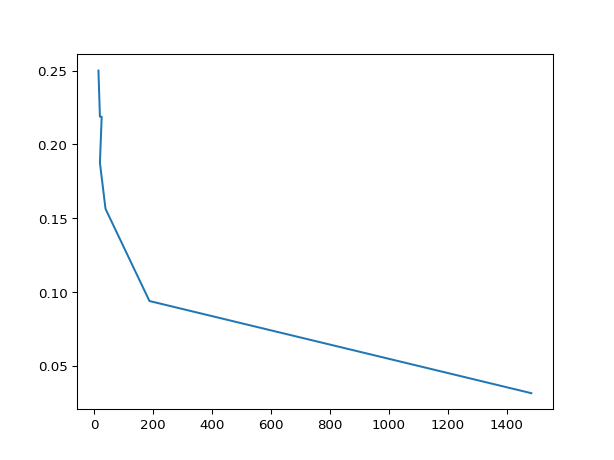
\includegraphics{plot.png}
    \caption{$\lambda_R$ Vs. $n$} \label{blah}
\end{figure}
\end{document}